\begin{savequote}
\quoteperson{Equations are just the boring part of mathematics. I 
  attempt to see things in terms of geometry.}{Stephen Hawking}
\end{savequote}

\chapter{Non-Euclidean Techniques}
\label{chap:noneuclid}

In this chapter we will extend the conformal model to cover non-Euclidean
geometries. Specifically, we shall fully develop a description of hyperbolic
geometry within the conformal model and show how a similar development may be
performed for spherical geometry.

Euclidean geometry, the geometry of the plane, was first defined\cite{Heath56} by
\emph{Euclid's Postulates}:

\begin{enumerate}
\item A straight line segment can be drawn joining any two points. 
\item Any straight line segment can be extended indefinitely in a straight line. 
\item Given any straight line segment, a circle can be drawn having the segment as radius and one endpoint as centre. 
\item All right angles are congruent. 
\item If two lines are drawn which intersect a third in such a way that the sum of the inner angles on one side is less than two right angles, then the two lines inevitably must intersect each other on that side if extended far enough.
\end{enumerate} 

This last postulate is equivalent to what is known as the \emph{parallel postulate},
which, loosely, states that two parallel lines will never meet, even at infinity.
In this chapter we shall explore hyperbolic geometry, one of the simplest
geometries that satisfy all but this last postulate.

%Ignoring the last postulate may, initially, seem a purely intellectual exercise
%although the last postulate has never been proved to exist in real-space
%by experiment. Who is to say that parallel beams of light emitted from
%Earth won't eventually converge somewhere out by Andromeda? Indeed, the 
%`bending' effect upon light by large gravitational fields almost
%guarantee the convergence of some light beams.

% \section{Non-Euclidean Geometries}

\section{Hyperbolic Geometry}

Hyperbolic geometry is usually represented in two dimensions on the
\emph{Poincar\'e disc}. This is a unit disc centred on the origin
onto which all space is mapped. A metric is defined within the
disc\cite{GEOM:Brannan} along with a set of congruence transformations.
The boundary circle of the disc represents the points at infinity. Everywhere
outside the disc is inaccessible to the hyperbolic geometry. Straight lines,
called $d$-lines\cite{GEOM:Brannan}, are represented by circular arcs which
erupt normal to the boundary circle. Perhaps one of the most famous examples of this
geometry is given in Escher's \emph{Circle Limit} series of wood prints, an example of
which is re-created in figure \ref{fig:circlelimit}. In these prints infinite
tessellations of hyperbolic space are represented mapped to the Poincar\'e
disc and they show the circular nature of $d$-lines, although Escher was
unaware of the Poincar\'e disc model at the time the prints were made.

\begin{figure} \centering
\scalebox{0.6}{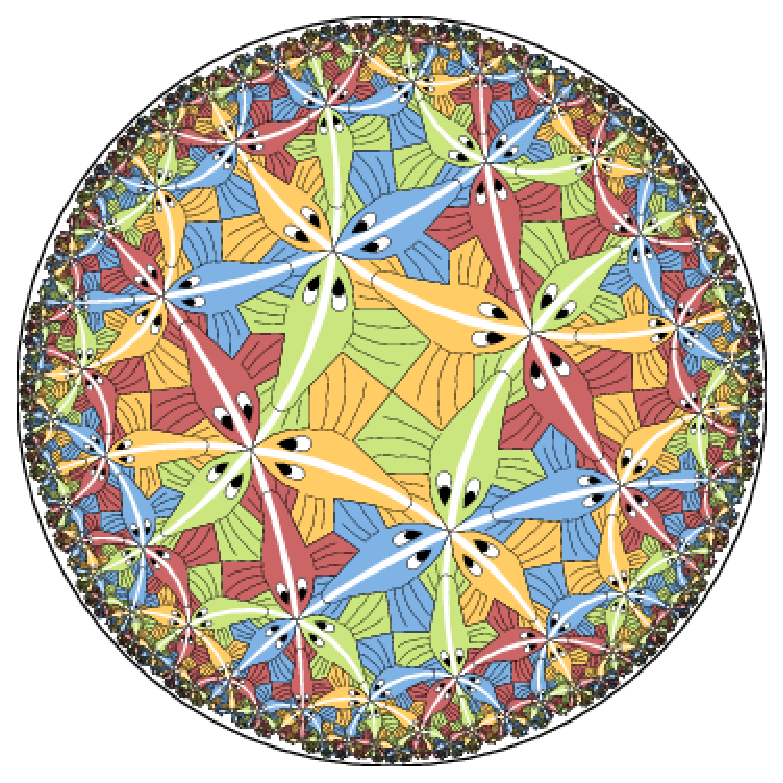
\includegraphics{circlelimit}}
\caption{A re-creation of Escher's \emph{Circle Limit III}, 
a depiction of hyperbolic geometry on the Poincar\'e disc.
Taken from \cite{transhyp}.}
\label{fig:circlelimit}
\end{figure}

\section{Extending the Conformal Model}
\label{sec:extendconfmodel}

In this section we shall extend the conformal model we have developed to
represent Euclidean geometry to the hyperbolic geometry of the Poincar\'e
disc and show how many results which are tedious to prove using existing
metric-based derivations become simple and, in some cases, obvious using the
GA-based approach.

All rigid-body transformation (i.e.\ rotation and translation) rotors in 
the Euclidean approach described in previous chapters leave $n$ invariant, i.e.\ 
$Rn\tilde{R} = n$ for all such rotors $R$. They also leave $\bar{n}$ invariant. We have
already identified $n$ and $\bar{n}$ with the points at infinity and the origin 
respectively. We shall now show that, since a geometry may be defined by its 
congruence transformations, changing which vectors are left invariant by rotors
will produce a different geometry.

Suppose we choose to restrict the rotors such that they keep $e$
invariant. Without loss of generality, we deal with a conformal extension of
$\mathbb{R}^2$ and write down a set of four basis vectors
\begin{equation}
E_1 = e_1 \quad E_2 = e_2 \quad E_3 = e \quad E_4 = \bar{e}
\end{equation}
and thus form the rotors $R_{k\ell } = \exp\left(\frac{\alpha}{2}E_k \wedge E_\ell\right)$ with $k,\ell \in \{1,2,3,4\}$.
Applying them to $e$ via $R_{k\ell }e\tilde{R}_{k\ell } \equiv R_{k\ell }eR_{\ell k}$, we find
the bivector generators of the rotors which preserve $e$ are $\bar{e}e_1$, 
$\bar{e}e_2$ and $e_1e_2$. The latter just correspond to rotations in the
$e_1e_2$ plane and hence, the former two must be the generators of
translations. We propose, therefore, that a rotor which translates the origin to the vector
$x$ must be given by a multivector of the form
\begin{equation}
T_x = \exp\left(\frac{f(r)}{2}\bar{e}\hat{r}\right)
\end{equation}
where $r = |x|$, $\hat{r} = x/|x|$ and $f(r)$ is some function of $r$ yet to
be determined. Noting that $(\bar{e}{e_1})^2 = (\bar{e}e_2)^2 = +1$ and therefore
$(\bar{e}\hat{r})^2 = +1$ we can take the power series expansion of $T_x$ and
collect like-coefficients to obtain
\begin{equation}
T_x = \cosh\left(\frac{f(r)}{2}\right) + \bar{e}\hat{r}\sinh\left(\frac{f(r)}{2}\right)
\label{eqn:nonEuclidTrans1}
\end{equation}

We now consider how to represent the origin. Our choice is restricted in 
that the origin must differ from the 
point at infinity and, to retain isotropy, must not contain components
parallel to $e_1$ or $e_2$.  Either $n$ or $\bar{n}$ would be a suitable
choice to investigate but we choose a multiple of $\bar{n}$ to retain
compatibility with the Euclidean case.

As with the Euclidean case we wish to impose a normalisation condition 
on the null-vectors, 
$X = F_e(x)$, such that 
\begin{equation}
X \cdot e = -1
\end{equation}
where we use $F_e(x)$ to represent the mapping defined by the geometry
generated by the rotors which
preserve $e$. We would also prefer if we could contain some 
relation to our mapping for Euclidean geometry. Hence we continue by
specifying that the origin is represented by null-vectors parallel to $-\bar{n}$.
% If this is to hold then the origin must in fact be $-\bar{n}$.

We can now find the representation of the general point $x$ as the translation
along $x$ of the origin. Writing $c = \cosh\left(\frac{f(r)}{2}\right)$ and
$s = \sinh\left(\frac{f(r)}{2}\right)$
\begin{eqnarray}
F_e(x) & = & T_x\,(-\bar{n})\,\tilde{T}_x \\
& = & \left[c + \bar{e}\hat{r}s\right] (-\bar{n}) \left[c - \bar{e}\hat{r}s\right] \\
&=& -c^2\bar{n} + 2sc\hat{r} + s^2n.
\end{eqnarray}
Letting $C = \cosh(f(r))$ and $S = \sinh(f(r))$ giving $c^2 = (C+1) / 2$,
$s^2 = (C-1)/2$, $sc = S/2$ and hence
\begin{eqnarray}
F_e(x) & = & \frac{1}{2}n (C-1) - \frac{1}{2}\bar{n}(C+1) + S\hat{r} \nonumber \\
& = & \frac{1}{2} \left[ \, (C-1)n + 2S\hat{r} - (C+1)\bar{n} \, \right] 
% & = & \frac{1}{2} \left[ \, (\cosh(f(r))-1)n + 2\sinh(f(r))\hat{r} - (\cosh(f(r))+1)\bar{n} \, \right] 
\label{eqn:almost-X-rep} 
\end{eqnarray}
As required $(F_e(x))^2 = 0$ and $F_e(x) \cdot e = -1$.

It remains to choose a sensible form for $f(r)$. We seek to choose $f(r)$ such that
the representation $F_e(x)$ is similar to our Euclidean representation $F(x)$
since this will allow us to use many of the same techniques we developed for the
Euclidean case. We can re-write our Euclidean representation 
in terms of $r$ and $\hat{r}$ as
\begin{equation}
F(x) = \frac{1}{2\lambda^2}(r^2n + 2 \lambda r\hat{r} - \lambda^2\bar{n})
\label{eqn:nonEuclidMap1}
\end{equation}

If we wish that $F_e(x)$ be similar to $F(x)$ then we have the conditions
\begin{equation}
\frac{S}{C + 1} = \frac{\sinh(f(r))}{\cosh(f(r)) + 1} = \frac{r}{\lambda}
\label{eqn:rlambda}
\end{equation}
and
\begin{equation}
\frac{C-1}{S} = \frac{\cosh(f(r)) - 1}{\sinh(f(r))} = \frac{r}{\lambda}
\label{eqn:rlambda2}
\end{equation}
so the mapping function becomes
\begin{eqnarray}
F_e(x) &=& \frac{C+1}{2\lambda^2}\ [x^2n + 2\lambda x - \lambda^2 \bar{n}] \\
&=& \frac{\cosh(f(r)) + 1}{2\lambda^2}\ [x^2n + 2\lambda x - \lambda^2 \bar{n}]
\end{eqnarray}
which has a degree of similarity to the expression for $F(x)$. Further, 
assuming $r$ and $\lambda$ are positive, we can see from equation
\ref{eqn:rlambda} that $r < \lambda$ since $\sinh(A) < 1 + \cosh(A)$
for all $A$.

Given equations \ref{eqn:rlambda} and \ref{eqn:rlambda2}, we can eliminate
$\sinh(f(r))$ to give
\begin{equation}
\frac{\cosh(f(r)) -1}{\cosh(f(r)) + 1} = \frac{r^2}{\lambda^2}
\end{equation}
and hence $\cosh(f(r)) = (\lambda^2 + r^2)/(\lambda^2 - r^2)$. Substituting
into either \ref{eqn:rlambda} or \ref{eqn:rlambda2} gives
\begin{equation}
f(r) = \sinh^{-1}\left( \frac{2\lambda r}{\lambda^2 - r^2} \right)
\end{equation}
and hence we can form the following expressions for 
$\sinh(f(r))$ and $\cosh(f(r))$
\begin{equation}
\sinh(f(r)) = \frac{2\lambda r}{\lambda^2 - r^2} \quad \mbox{ and } \quad
\cosh(f(r)) = \frac{2\lambda^2}{\lambda^2 - r^2} - 1.
\label{eqn:sinhcosh}
\end{equation}

Inserting these into equation \ref{eqn:nonEuclidMap1} gives the final form
of the non-Euclidean mapping function
\begin{equation}
F_e(x) = \frac{1}{\lambda^2 - x^2}(x^2 + 2\lambda x - \lambda^2\bar{n})
\label{eqn:nonEuclidMapping}
\end{equation}

We can also show, by substituting the results in equation \ref{eqn:sinhcosh}, 
that the form of the translation rotor given in 
equation \ref{eqn:nonEuclidTrans1} can also be written as
\begin{equation}
T_x = \frac{1}{\sqrt{\lambda^2 - x^2}}(\lambda + \bar{e}x)
\label{eqn:transrotor}
\end{equation}

\begin{figure} \centering
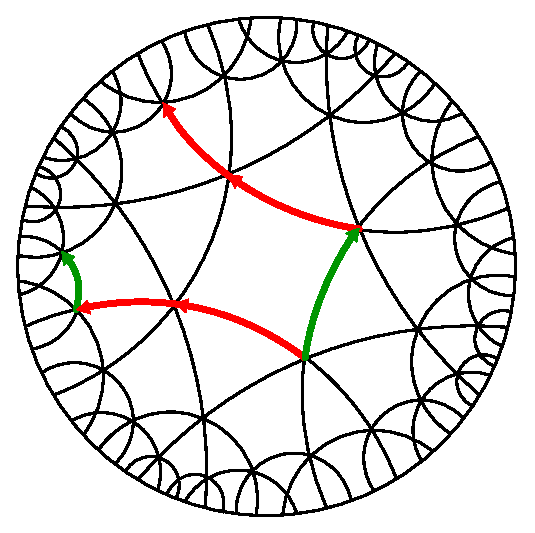
\includegraphics[width=0.9\columnwidth]{circlimitgrid}
\caption{An illustration of how translation, interpreted as movement along
geodesics, in hyperbolic geomtry is non-commutative.
\label{fig:limitgrid}}
\end{figure}

Some discussion of the relevance of $\lambda$ is worthwhile here. Notice that
in order for the translator to remain real-valued, $x^2 \le \lambda^2$. 
We can never therefore translate the origin outside of a circle radius
$\lambda$ centred upon it. The value of $\lambda$ gives the distance to
the boundary of a region of inaccessible space from the origin. It is
in effect a circular boundary to the geometry. This circle corresponds
directly to the unit-circle boundary in the Poincar\'e disc representation if
$\lambda = 1$ and simple dilations of the Poincar\'e representation if
$\lambda \ne 1$. To maintain compatibility with the Poincar\'e representation,
we usually set $\lambda$ to be unity.

The rotor in equation \ref{eqn:transrotor} is, by construction, the rotor 
which takes us from the origin to position $x$. Interestingly translations in
hyperbolic geometries do not commute; that is moving a position
vector $a$ along another vector $b$ does not, in general, give the same result
as moving $b$ along $a$. This can be seen by tracing the grid
in figure \ref{fig:circlelimit} as shown in figure \ref{fig:limitgrid}.
In this figure we translate along the vector drawn in red twice and translate
along the vector marked in green once. Depending on the order of application
we arrive at different locations.
It is therefore geometrically clear why,
unlike the Euclidean case, the hyperbolic translation rotors
$T_x$ and $T_y$ do not commute
for two different positions $x$ and $y$. 
It is alo clear algebraically since
\[
T_xT_y = \alpha(\lambda + \lambda\bar{e}(x+y) - \bar{e}xy\bar{e})
\]
\[
T_yT_x = \alpha(\lambda + \lambda\bar{e}(x+y) - \bar{e}yx\bar{e})
\]
which are only identical if $xy = yx$, i.e.\ if $x$ and $y$ are parallel.
This means that
$T_{y-x}$ is {\em not} the rotor taking us from
position $x$ to position $y$. However, this is not a
problem, since we can always achieve this motion via
going back through the origin, and forming
%
\begin{equation}
T_{x \mapsto y} = T_y T_{-x}
\end{equation}
%
Since composition of rotors always produces another
rotor, this means that we have the same freedom as in the
Euclidean case to prove a relation we are interested in,
at some special position and orientation, and then use
the covariant rotor structure to generalise the result to
general positions and orientations. Spatial rotations about the origin are
of course achieved as before with rotors of the form
$R=\exp\left(\frac{\theta}{2}e_1 e_2\right)$.

The final motion we should consider is the analogue of
inversion. Unlike in the Euclidean case, inversion using
reflection in $e$ is now a fully covariant operation.
Specifically, if $R$ represents any combination of
rotation and translation, and $A$ is some object in the
space, we have
%
\begin{equation}
eAe \mapsto Re\tilde{R}\, RA\tilde{R}\, Re\tilde{R} = e
RA\tilde{R} e = R(eAe) \tilde{R}
\end{equation}
%
The last equality means that transforming $A$ first and
then reflecting is the same as reflecting and then
transforming, which is what is required of a covariant
operation. The availability of this reflection operation
is very useful. The translation rotors discussed above
clearly only allow us to move around within the interior
of the disc $r<\lambda$. By reflection in $e$, as we
shall see below, we are able to jump into a `dual world'
outside the disc.

Having achieved a representation function, and discussed
the set of motions, we should examine this new space in
relation to the Poincar\'e disc, which we have claimed it is
equivalent to with a view to justifying this claim.
To do this we shall examine the distance
function, i.e. how we assign a non-Euclidean distance
function between points in the space.

If we consider a simple rotation,
$\exp\left(\frac{\theta}{2}\hat{B}\right)$, where $\hat{B}$ is some unit
spatial bivector, then we are used to the idea that
$\theta$ is the correct measure of distance (here
angular) to describe the transformation. Thus if we
consider again the translation rotor in
equation \ref{eqn:nonEuclidTrans1}, $T_x = \exp\left(\frac{f(r)}{2}\bar{e}\hat{r}\right)$,
%
%\begin{equation}
%T_x = \cosh(f(r)/2) + \ebar \rhat \sinh(f(r)/2) =
%\exp((f(r)/2) \ebar\rhat)
%\end{equation}
%
%where $f(r) = \sinh^{-1}\left(\frac{2\lambda
%r}{\lambda^2-r^2}\right)$,
we would expect the correct distance
measure to associate with it would be $f(r)$. This would be a
viable option, except that for points close to the origin of the
disc ($r\ll\lambda$) we would like ordinary Euclidean notions of
distance to apply, at least approximately. It is clear that $\ebar =
(1/2)(n-\nb)$ and the $\nb$ part of this, when exponentiated and
applied as in equation \ref{eqn:almost-X-rep}, has no effect to
first order on the origin point $-\nb$, whereas the $n$ part does,
i.e.
%
\begin{eqnarray}
T_x(-\nb)\tilde{T}_x & \approx  & \left(1+
\frac{f(r)}{2}\frac{(n-\nb)\rhat}{2}\right)(-\nb)\left(1-
\frac{f(r)}{2}\frac{(n-\nb)\rhat}{2}\right)   \nn \\
 & =  &
\left(1+
\frac{f(r)}{2}\frac{n\rhat}{2}\right)(-\nb)\left(1 -
\frac{f(r)}{2}\frac{n\rhat}{2}\right).
\end{eqnarray}
%
This means that, to first order near the origin, the
$T_x$ rotor approximates in its actions the Euclidean
translation rotor corresponding to distance $f(r)/2$
rather than $f(r)$, i.e.
%
\begin{equation}
T_x \approx 1 + \frac{f(r)}{2}\frac{n \rhat}{2}
\end{equation}
%
For this reason, we take the non-Euclidean distance
between a point and the origin to be given by $f(r)/2$
rather than $f(r)$. Calling this non-Euclidean distance
function $d(r)$, and using equation
\ref{eqn:sinhcosh} along with the identity 
\[\sinh\left(\frac{z}{2}\right) =
\left[\frac{\cosh z - 1}{2}\right]^{\frac{1}{2}},\]
gives
%
\begin{equation} \label{eqn:defines-dofr}
d(r) =
\sinh^{-1}\left(\frac{r}{\sqrt{\lambda^2-r^2}}\right)
\end{equation}
%
We note this approximates to $r/\lambda$ for
$r\ll\lambda$, i.e.\ we recover the Euclidean distance
measured in units of $\lambda$.

This function gives us the distance of a point from the
origin, but what about the distance between two general
points, neither of which is at the origin? One of the
major advantages of the conformal approach to Euclidean
geometry is that it gives us an inner product formula for
computing the distance between any two points, and we
would hope that the same would be possible here. This is
indeed the case. Let $X$ be the null vector corresponding
to the point $x=r\, \rhat$ using our representation,
equation (\ref{eqn:nonEuclidMap1}). Then, since $n\dt\nb =
2$, we can rewrite equation \ref{eqn:defines-dofr} as
%
\begin{equation} \label{eqn:dist-to-origin}
d(r) = \sinh^{-1}\left(\sqrt{-\frac{1}{2} X \dt (-\nb) }
\right)
\end{equation}
%
Note, $X \dt (-\nb)$ is the inner product of $X$ with the
null vector representing the origin. Two points in any
general positions can be wound back using a common
translation rotor so that one of them ends up at the
origin. For example, let $T_y$ be the translation rotor
that takes $Y$ back to the origin, then
%
\[ X' = T_y X \tilde{T}_y \qquad  Y' = T_y Y \tilde{T}_y
= -\nb
\]
%
so that $X'\dt Y' = (T_y X \tilde{T}_y)\dt T_y Y \tilde{T}_y =
X\dt Y =  X'\dt (-\nb)$. Since we know that a function of $-\half
X'\dt (-\nb)$ gives the distance between the two points from
equation~(\ref{eqn:dist-to-origin}), we can now write this
distance in terms of $X\dt Y$. Note that at no stage in the
process has the inner product between the null vectors changed (the
inner product is rotor invariant), and thus we have succeeded in
defining a distance between general points in terms of inner
products. If the general points are $x$ and $y$ with
representatives $X$ and $Y$, the expression for the distance
function is thus
%
\begin{equation}\label{eqn:general-dist-formula}
d(x,y) = \sinh^{-1}\left(\sqrt{-\frac{1}{2} X \dt Y }
\right)
\end{equation}
%
which is a satisfyingly simple relationship. As in the
Euclidean case, it is a monotonic function of $X\dt Y$.
If we take the inner product of $X$ and $Y$ we obtain,
using equation~\ref{eqn:nonEuclidMap1},
%
\begin{eqnarray}
X\dt Y  & = &
\frac{1}{(\lambda^2-x^2)(\lambda^2-y^2)}\left[-2\lambda^2x^2-2\lambda^2y^2+4\lambda^2xy\right] \nn \\
  &  =  &
  \frac{-2\lambda^2}{(\lambda^2-x^2)(\lambda^2-y^2)}(x-y)^2
  \end{eqnarray}
%
Written in terms of the points themselves the distance
between the points is therefore
%
\begin{equation}\label{eqn:general-dist-formula-points}
d(x,y) = \sinh^{-1}\left(\lambda
\sqrt{\frac{(x-y)^2}{(\lambda^2-x^2)(\lambda^2-y^2)} }
\right).
\end{equation}
%

Armed with this distance function, we can now investigate
geodesics in the disc. These are the lines that are `straightest'
in the geometry defined by the distance function (more precisely,
the arc length along them is extremal.) We will not give the
details, but show some numerically computed examples in
figure~\ref{fig:hyper-geos}.
%
\begin{figure} \label{fig:hyper-geos}
\centerline{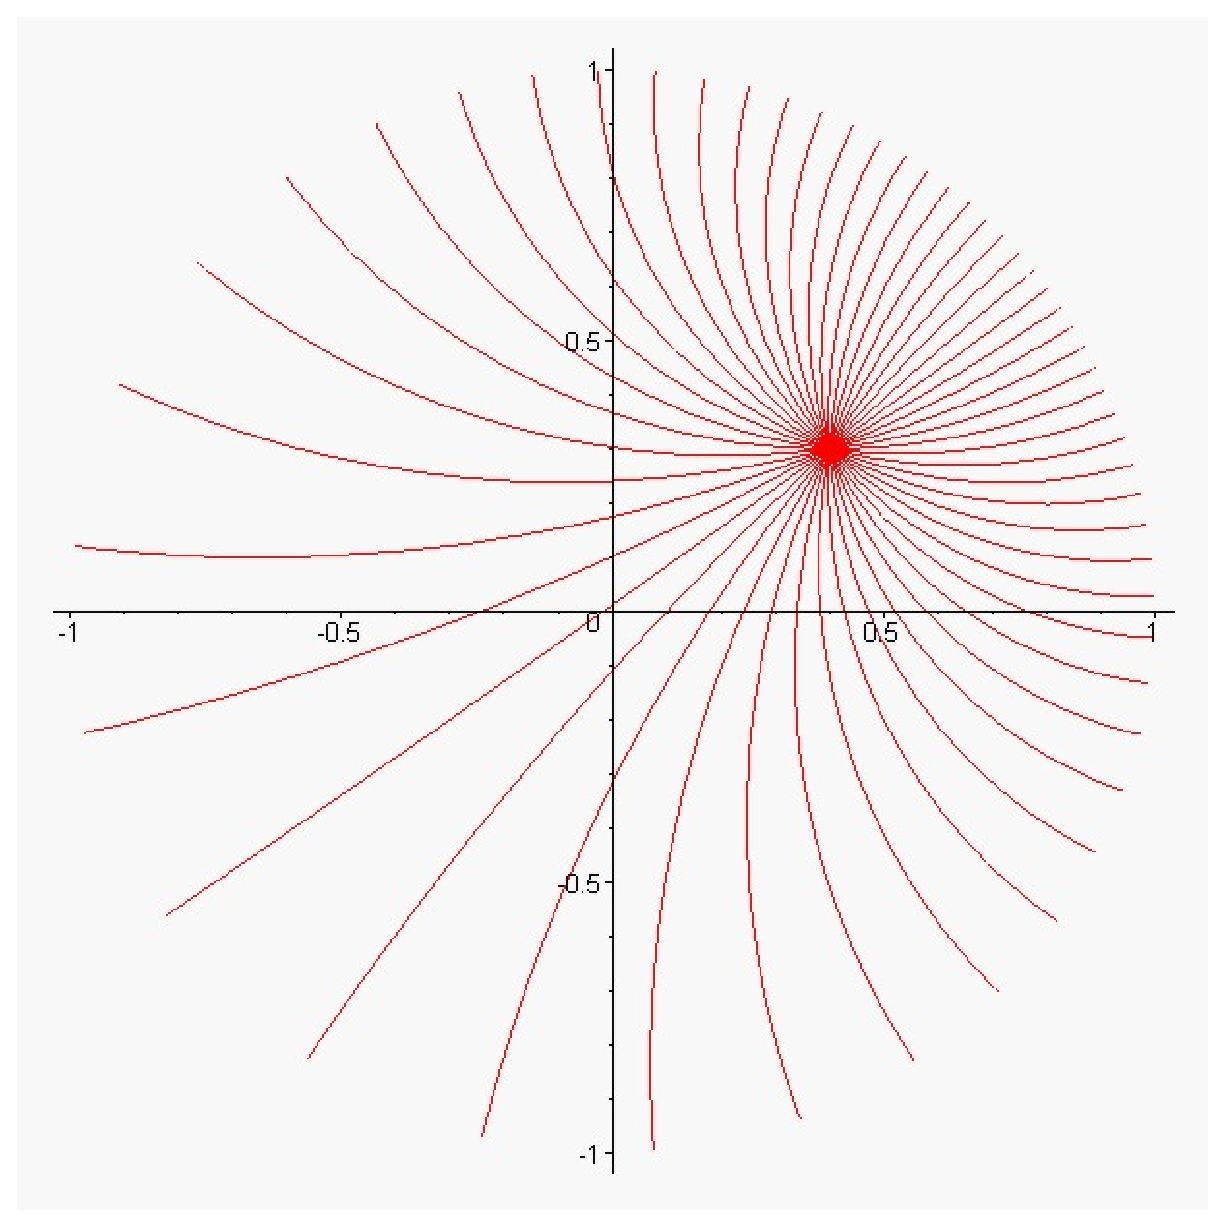
\includegraphics[width=0.9\textwidth]{hyper_geos}}
\caption{Geodesics eminating from a point in hyperbolic space.
They all intersect the unit circle at right angles and each is in
fact the arc of a circle. ($\lambda=1$ has been taken here.) }
\end{figure}
%
In calculating these we have taken $\lambda=1$, so the disc is now
the unit disc ordinarily considered in the Poicar\'e model. One
finds that each geodesic is an arc of a circle, and that each of
them asymptotically approaches the bounding unit circle at right
angles. At this point we can start making contact with the
description of the classical approach to the Poincar\'e
disc\cite{GEOM:Brannan}. The geodesics there are called {\em $d$-lines}.
They are not justified in terms of being geodesics, but simply
defined as being arcs of circles which cut the boundary at right
angles. However the distance function given in \cite{GEOM:Brannan}
in terms of distance to the origin is
%
\begin{equation}
d(x,0) = \tanh^{-1}(|x|)
\end{equation}
%
and therefore agrees with our identification of $d(r)=
f(r)/2$, using equation \ref{eqn:sinhcosh}, and
taking $\lambda=1$.

This distance function allows us to define a geometrically analogous
dilator about the origin. Suppose we dilate some vector $x$ about the
origin so that $x \mapsto x'$. We would expect that, given a dilation
factor of $a$, $d(x',0) = a\,d(x,0)$ or, equivalently,
\begin{eqnarray*}
\tanh^{-1}(|x'|) = a \tanh^{-1}(|x|) \\
|x'| = \tanh[ a \tanh^{-1}(|x|) ] \\
\frac{|x'|}{|x|} = {\tanh[ a \tanh^{-1}(|x|) ]}({|x|})^{-1}.
\end{eqnarray*}
We see that a hyperbolic dilation by a factor of $a$ is therefore
equivalent to an Euclidean dilation by ${\tanh[ a \tanh^{-1}(|x|) ]}({|x|})^{-1}$.

Thus far, apart from the formula for non-Euclidean
distance in terms of $X \dt Y$, we have only mirrored
what is already known. We now start to show the power of
the conformal GA approach to this geometry, by showing
how the operations and objects defined previously in
conformal Euclidean geometry have immediate analogues
here, representing a considerable unification, and saving
of effort. It may also be worth noting here that the
power of this approach extends immediately to three or more
dimensions where the Poincar\'e
disc becomes a sphere. On the other hand, to provide a
computational scheme which is somewhat akin to our rotor
formulation, Brannan \emph{et al} \cite{GEOM:Brannan} introduce complex coordinates
to work in the Poincar\'e disc, and use Mobius
transformations in place of the rotors. These are
effective computationally in two dimensions, but of course the
complex variable apparatus does not extend at all to three dimensions.
Also the
conformal setup enabling points, lines, circles, spheres
and planes to be integrated into one algebraic system
does not exist in the complex variable approach, even in
two dimensions.

\subsection{Geometric Objects in Hyperbolic Geometry}

In this section we shall develop representations for geometric objects
within hyperbolic geometry as we did previously for Euclidean geometry.

\subsubsection{Hyperbolic lines}

Having dealt with distances between points, let us start with the
next most fundamental objects --- lines. In Euclidean space we
have seen that these are given by $L = n \wedge A \wedge B$, where $A$
and $B$ are the representatives of any two points on the line.
Rotor transformations are able to move lines around successfully
because for either a rotation or translation, $R n \tilde{R} = n$.
Thus when we perform $R L \tilde{R}$ we end up with $n \wedge (R A \tilde{R})
\wedge (R B \tilde{R})$ which is a line through the transformed points.
Dilations also fit into this, since although they introduce a
scale factor when acting on both $n$ and general points, this
still produces the intended line up to a scale factor in the
Euclidean case.

This discussion makes it clear what a line must be in the
conformal approach to hyperbolic geometry. Instead of
using $n$, we must use the invariant object $e$. Thus we
define a hyperbolic line as
%
\begin{equation}\label{eqn:line-def}
L = e \wedge A \wedge B
\end{equation}
%
where $A$ and $B$ are the two points through which we
wish it to pass. This construction will guarantee
covariance of the definition of a line, for the same
reasons as in the Euclidean case (namely here that $R e
\tilde{R} = e$ for any allowable rotor $R$).

The immediate, very important question, of course, is
what precisely {\em is\/} the object we have constructed.
Ideally it should correspond to the $d$-line geodesics we
have just discussed. To determine whether a position $X$
lies on this line, we need to solve $X\wedge L=0$. Let us
take $x=x_1 e_1 + x_2 e_2$, $a=a_1 e_1 + a_2 e_2$ and
$b=b_1 e_1 + b_2 e_2$. Then, taking $\lambda=1$ for
convenience,  it is easy to show the resulting equation
for $x$ is of the form
%
\begin{equation}\label{eqn:brannan-d-line}
x_1^2+x_2^2-2 p x_1 -2 q x_2 +1 =0
\end{equation}
%
where $p^2+q^2>1$. Specifically, one finds
%
\begin{align}
p &= -\frac{1}{2}\,\frac {\left\{({a_1}^2+{a_2}^2
+1)\,b_2 - ({b_1}^2+{b_2}^2 +1)\,a_2\right\}}{ a_1\, b_2-
a_2\, b_1} \nn \\
%
q &= -\frac{1}{2}\,{\frac {\left\{-({a_1}^2+{a_2}^2
+1)\,b_1 + ({b_1}^2+{b_2}^2 +1)\,a_1\right\}}{{ a_1}\,{
b_2}-{ a_2}\,{ b_1}}} \nn
%
\end{align}
%
Equation \ref{eqn:brannan-d-line} is precisely the form
of equation given for $d$-lines in Brannan \emph{et al}\cite{GEOM:Brannan} 
page 283 and shows that
indeed our recipe in terms of wedging with $e$ has worked.

We can combine the notions of lines and distance, by asking for
the `hyperbolic midpoint' of the line segment joining two
positions $a$ and $b$. This is that point lying on the $d$-line
between $a$ and $b$ which is an equal hyperbolic distance from
each. Brannan \emph{et al}\cite{GEOM:Brannan} deal with this on page 288, but
consider only the easiest case where the two points lie along a diameter of
the unit disc.

We know in the Euclidean case, that forming $A+B$ will give a
non-null point consisting of a multiple of the null vector
representing the desired midpoint, plus a multiple of the point at
infinity $n$. We hypothesise that we will get the same behaviour
here, but with $e$ playing the role of $n$. We can use two
different methods to obtain these results. The second is faster
than the first, but we outline both, since they both typify the
techniques available for use, and serve as good illustrations of
the power of the covariant method for hyperbolic geometry.

Firstly, since we can move objects around at will, let us
establish the result in the simplest case, where the two
points are symmetrically disposed about the origin, e.g.
let $a=\alpha e_1$ and $b=-\alpha e_1$. Clearly, by
symmetry the hyperbolic midpoint must be the origin
itself, so we write
%
\begin{equation} \label{eqn:mid-point-requirement}
A+B = \beta (-\nb) + \delta e
\end{equation}
%
where $\delta$ and $\beta$ are scalar multiples to be determined.
Since $A+B = \frac{2}{\lambda^2 - \alpha^2}(\alpha^2 n - \lambda^2
\nb)$ it is easy to see that we must have
%
\begin{equation}
\delta = \frac{4\alpha^2}{\lambda^2-\alpha^2} \quad
\text{and} \quad \beta =
\frac{2(\alpha^2+\lambda^2)}{\lambda^2-\alpha^2}
\end{equation}
%
Meanwhile, we note that
%
\begin{equation}
A\dt B = -\frac{8 \alpha^2
\lambda^2}{(\lambda^2-\alpha^2)^2}
\end{equation}
%
and some straightforward manipulation then tells us that
%
\begin{equation} \label{eqn:delta-beta-results}
\delta=\sqrt{4-2 A\dt B} -2 \quad \text{and} \quad \beta
= \sqrt{4-2 A\dt B}.
\end{equation}
%
%We have by this means actually solved the general
%problem! To see this, note that we can now rearrange
%equation (\ref{eqn:mid-point-requirement}) to get
We may solve the more general problem by rearranging 
equation \ref{eqn:mid-point-requirement} to get
%
\begin{equation}
-\nb = \frac{1}{\sqrt{1-\frac{1}{2} A \dt B}} \left\{
\frac{1}{2} (A+B) - e \left(\sqrt{1-\half A \dt
B}-1\right) \right\}
\end{equation}
%
Everything on the right hand side is covariant, and the separation between
$A$ and $B$ was controlled by a variable which was kept general
($\alpha$), so by employing translation and rotation rotors on the
right hand side we can make $A$ and $B$ line up with any two desired
points. Meanwhile the left hand side will keep track, and must still
remain the midpoint. To see this, note that its `dot' with the
new points that $A$ and $B$ transform into, will remain constant
during this process. The $e$ term just remains invariant. For two
completely general points $A$ and $B$ therefore, their
hyperbolic midpoint is given by
%
\begin{equation} \label{eqn:mid-point-expr}
X_{\rm mid} = \frac{1}{\sqrt{1-\frac{1}{2} A \dt B}}
\left\{ \frac{1}{2} (A+B) - e \left(\sqrt{1-\half A \dt
B}-1\right) \right\}
\end{equation}
%
which is a fully covariant expression.

The alternative method, which is easier computationally, is as
follows. Let us write equation \ref{eqn:mid-point-requirement}
again but this time with $X_{\rm mid}$ in place of $-\nb$ and with
a general $A$ and $B$ in place from the beginning. So
%
\begin{equation}
A+B = \beta \, X_{\rm mid} + \delta e
\end{equation}
%
Rearranging, we have
%
\begin{equation}
X_{\rm mid} = \frac{1}{\beta} (A+B-\delta e)
\end{equation}
%
which shows that our assumption about the form of the
midpoint is in fact valid. This is because dotting the
right hand side with $A$ and $B$ in turn, we obtain
%
\begin{equation}
X_{\rm mid} \dt A = X_{\rm mid} \dt B = \frac{1}{\beta}
(A\dt B+\delta)
\end{equation}
%
This means that $X_{\rm mid}$ is indeed equidistant, in a
hyperbolic sense, from $A$ and $B$. Moreover,
%
\begin{equation}
X_{\rm mid} \wedge (e \wedge A \wedge B) = 0
\end{equation}
%
so it correctly lies on the $d$-line joining them.

It just remains to fix $\delta$ and $\beta$ via requiring
that $X_{\rm mid}$ is null and is correctly normalised.
The null requirement gives
%
\begin{equation}
2 A \dt B + 4 \delta + \delta^2 = 0
\end{equation}
%
and requiring $X_{\rm mid} \dt e = -1$ yields
%
\begin{equation}
\beta=\delta+2
\end{equation}
%
Solving these yields equation \ref{eqn:delta-beta-results} as
before, and we recover equation \ref{eqn:mid-point-expr}.

\subsubsection{Hyperbolic circles}

A great deal of hyperbolic geometry is concerned with
hyperbolic circles, i.e. the locus of points that are
at a constant hyperbolic distance from a given centre.
We can immediately hypothesise that such a circle,
passing through the points $A$, $B$, $D$  should be given
by the trivector.
%
\begin{equation}
C = A \wedge B \wedge D
\end{equation}
%
The set of points $X$ which satisfy $X\wedge C=0$ can be found
in a similar manner to the Euclidean case since the null-vector
representation is the same up to a scale factor; 
i.e.\ in the Euclidean case we know that $X =
\frac{1}{2\lambda^2}[x^2n + 2\lambda x - \lambda^2\nb]$ and in the
hyperbolic case $X = \frac{1}{\lambda^2 - x^2}[x^2n + 2\lambda
x - \lambda^2\nb]$.
If the above hypothesis is true, we can
immediately deduce the somewhat surprising, though in fact true,
conclusion that hyperbolic circles are also Euclidean circles.
It turns out that it is just their centres that are in general
different.

To establish that $C$ is a hyperbolic circle, as well as
clearly a Euclidean one, we can take the special case of a circle
centred at the origin. By symmetry, this must be both a Euclidean
and hyperbolic circle. Let this have Euclidean radius $\rho$.
If we recall our earlier work, then for the scaled version of the
null point representative, the inner product between two points
$A$ and $B$ is given by
%
\begin{equation}
     A\dt B = -\frac{1}{2\lambda^2}(a-b)^2
     \end{equation}
%
Then, since $X\dt B = -\frac{1}{2\lambda^2}(x-b)^2 =
-\frac{1}{2\lambda^2}(\rho)^2$ for a circle centre $B$ and radius
$\rho$, we have that
%
\begin{equation}
  X\dt (B-\frac{1}{2\lambda^2}(\rho)^2n)=0
\end{equation}
%
giving $C^*=B-\frac{1}{2\lambda^2}(\rho)^2n$, where $C$ is the
trivector describing the circle. Thus if $B$ is the origin, so
that $B = -\frac{1}{2}\nb$, the dual of $C$ is given by $C^* =
-\frac{1}{2\lambda^2}\{\rho^2 n + \lambda^2\nb\}$. Now, since
$n+\nb = 2e$ we can write $\rho^2 n + \lambda^2\nb$ as
%
\begin{equation} \label{eqn:dual-to-C}
\rho^2 n + \lambda^2 \nb = 2 \rho^2 e + (\lambda^2 -
\rho^2) \nb
\end{equation}
%
We can normalise this to $C^2=(C^{*})^2=1$ via the scaling
\[C^* \mapsto \alpha(\rho^2n + \lambda^2\bar{n})\quad\mbox{such that}
\quad(C^{*})^2 = 1
\]
and hence $\alpha = \frac{1}{2\rho\lambda}$, thus
\begin{equation}
C^* = \frac{1}{2 \rho \lambda} \left(\rho^2 n + \lambda^2 
\nb\right)
		=
\frac{1}{2\rho\lambda}[2\rho^2e + (\lambda^2 - \rho^2)\bar{n}].
\end{equation}
%
This displays the dual to $C$ as a linear combination of
the vector representing the origin, which is here the
centre of the circle, and a multiple of $e$. This is the
covariant form we require for generalisation. Note
%
%
\begin{equation}
X \dt (IC) = \frac{1}{2 \rho \lambda} \left\{ X \dt (2 \rho^2 e +
(\lambda^2 - \rho^2) \nb) \right\} = \frac{1}{2 \rho \lambda}
\left\{ -2\rho^2 -(\lambda^2-\rho^2) X \dt (-\nb) \right\}
\end{equation}
%
shows us how $X$ maintaining a constant hyperbolic distance
from the centre ($-\nb$) is guaranteed by $X \dt (IC)=0$, in which
case we have
%
\begin{equation}
X \dt (-\nb) = \frac{-2\rho^2}{(\lambda^2 - \rho^2)}.
\end{equation}
%
Let us act on $IC=I(A \wedge B \wedge D)$ with hyperbolic rotors,
to move the 3 points around as we wish. These same rotors acting
on the right hand side of equation \ref{eqn:dual-to-C} mean that we will
continue to get the required behaviour of constant hyperbolic
distance from the transformed centre, since the rotors will take
the origin to the new centre of the circle, say $P$. Thus indeed,
the wedge of 3 points generates a hyperbolic circle, and
moreover the above enables us to extract its (hyperbolic)
radius and centre from the dual object. Again we see that the
r\^ole of the $n$ appearing in the Euclidean expressions is
replaced by $e$ here. Specifically we find the following: the
(normalised dual to the) hyperbolic circle with hyperbolic
centre $P$, Euclidean radius $\rho$ and hyperbolic radius $d$,
is given by
%
\begin{equation}\label{eqn:non-e-circle}
IC = \frac{1}{2 \rho \lambda} \left( 2 \rho^2 e +
(\rho^2-\lambda^2) P \right)
\end{equation}
%
with $d= \sinh^{-1} (\rho/\sqrt{\lambda^2-\rho^2})$, from
equation~\ref{eqn:general-dist-formula}.

\subsubsection{Hyperbolic reflection}

A very useful operation in hyperbolic geometry is the notion of
hyperbolic reflection as defined, for example, in \cite{GEOM:Brannan}. 
It is extremely easy to calculate the hyperbolic
reflection of a point $X$ in the $d$-line $L$ in the GA approach.
Assuming $L$ is normalised to satisfy $L^2=1$, we just form $LXL$,
the standard form of reflecting one object in another. Since $L e
L = e$ for any normalised line, we see that $X'=LXL$ is both
null and satisfies $X' \dt e=-1$ thus qualifying it to represent a
point. Moreover it is covariantly constructed;
under a rotor transformation it just rotates to $R X'
\tilde{R}$ and thus must represent something physical. It is not
hard to show that the point it represents is that found by moving
along a $d$-line intersecting $L$ at right angles and passing
through $X$, by an equal hyperbolic distance on the other side
of the line as $X$ is on the original side. This is indeed the
definition of reflection in this case.

\subsection{Extension to Higher Dimensions and Other Geometries}

All the above transfers seamlessly to three and higher dimensions, in
most cases with no changes at all to the formul\ae. This is in
contrast to e.g. the methods introduced in \cite{GEOM:Brannan}, which
rely on standard complex analysis and so only work in the 2d
plane. Furthermore, we can extend all the above analysis to the
case of \textit{spherical geometry} as well. This involves
replacing the role of $e$ with that of $\bar{e}$, which changes
some trigonometric functions and ranges of applicability, but
otherwise most of the above discussion goes through unchanged.

% \subsection{Space-Time Algebra}

\section{Non-Euclidean Visualisation Methods}
\label{sec:noneuclid-vis}

A key requirement for visualising objects in the Poincar\'e disc
representation of hyperbolic geometry is to plot representations of
straight lines, known as $d$-lines. This section outlines a method 
developed to draw them using OpenGL and also presents a generalisation
of the method for drawing analogous `$d$-planes' in three-dimensional
hyperbolic geometry.

\subsection{NURBs}

The $d$-lines on the Poincar\'e disc are circular arcs (and straight lines
for the special cases of lines through the origin). OpenGL, the graphics
library used for the implementation, has native support for a class
of curves called Non-uniform Rational B-Splines (NURBS)\cite{mecg}. 

%It is
%not the r\^ole of this report to provide a complete tutorial on NURBS,
%suffice it to say that they provide a way of parametising a large class of
%curves by a set of \emph{control points} and associated \emph{weights}.

NURBS curves are specified using a set of control points, $P_i$,
weights, $w_i$ and a set of normalised basis functions $N_{i,k}$.
The curve is given by
\[
C(u) = \frac{\sum_{i=0}^n w_i P_i N_{i,k}(u)}{\sum_{i=0}^n w_i N_{i,k}(u)}
\]

The basis functions are defined recursively:
\[
N_{i,k}(u) = \frac{u - t_i}{t_{i+k} - t_i} N_{i,k-1}(u) +
  \frac{t_{i+k+1} - u}{t_{i+k+1} - t_{i+1}} N_{i+1,k-1}(u)
\]
with
\[
N_{i,0} = 
\begin{cases}
1 \mbox{ if } t_i \le u \le t_{i+1} \\ 
0 \mbox{ otherwise} 
\end{cases}
\]
and $t_i$ being the elements of the \emph{knot vector}
\[
U = \{ t_0, t_1, ... , t_m \}
\]

The relation between the number of knots, $m+1$, the degree $k$ of 
the functions $N_{i,k}$ and the number of control points, $n+1$
is given by $m = n + k + 1$ \cite{peigl, rogers}.

Clearly a large family of curves can be expressed with suitable choices
of knot vectors, weights and control points leading to great flexibility.
All NURBS curves share some common properties however which make them
useful in Computer Graphics. A NURBS curve \emph{always} stays inside the
convex hull of its control points \cite{rogers} and thus it is straightforward
to compute whether the curve will be displayed at all. Further they
are tangential to the piece-wise linear interpolation of control
points at the end-points as illustrated in figure \ref{fig:samplenurb}.

\begin{figure} \centering
\scalebox{0.9}{\includegraphics{samplenurb}}
\caption{A set of control points and a typical example of an associated
NURBS curve. Note that the endpoints of the curve are tangential to
$P_0P_1$ and $P_5P_6$ and that the curve is within the convex hull
of the points (shaded).}
\label{fig:samplenurb}
\end{figure}

\subsection{Rendering $d$-lines}

To draw $d$-lines on the Poincar\'e disc, we wish to draw circular arcs
with end-points on the boundary circle and erupting normal to it.

A large number of different curves can be created with different control 
point numbers, positions and weights. Fortunately there are a number of
standard techniques to generate common curves. One such method of
drawing circular arcs\cite{NURBS:arc} is useful to us. We use three control
points; one at the start of the circular arc, one at the origin of the
boundary circle and one
at its end, see figure \ref{fig:nurbs}. 
The end-point weights are unity whereas the weight of the control
point at the origin is $\cos \gamma$ where $\gamma$ is the angle
$OA$ makes with $AB$.

\begin{figure} \centering
\scalebox{0.7}{\includegraphics{nurbs}}
\caption{NURBS-based rendering of $d$-lines. Here $O$ is the origin and
$A$ and $B$ are the boundary points of the line $L$.}
\label{fig:nurbs}
\end{figure}

Since NURBS are tangential to the piecewise linear interpolation of control 
points
at either end, it is clear that the curve erupts from the boundary
tangential to the lines $OA$ and $OB$. Given $O$ is the origin, and the
boundary is centred upon it, these lines are radii of the boundary
circle and so clearly are normals.

This allows us to construct a NURBS representation of any $d$-line
on the Poincar\'e disc (including diameters) and efficiently draw them
using OpenGL. 

\subsubsection{Calculating properties of $d$-lines}

The last step in drawing our $d$-lines is now finding where they intersect
the boundary disc, their \emph{boundary points}. 
Once we have these points, the drawing can be performed
via our NURBS-based method outlined above.

We can calculate boundary points of $d$-lines
by forming a circle 
corresponding to the boundary and finding the 
meet of the line with this circle. This gives the null-vector
representation of the boundary points $A$ and $B$ as the
bivector $A \wedge B$ as with circle/sphere intersections and the like.
We have already shown that this bivector can be factorised into $A$ and 
$B$ via the method of projectors.
We finally need to calculate the angle $\gamma$ which is a trivial
exercise in trigonometry.

Figure
\ref{fig:hyp1} shows the rendering of $d$-lines in action.
Here we have three $d$-lines created by rotating and translating the
diameter to form a hyperbolic triangle (central dark-shaded
region). Each of these lines was then reflected in the other two to form 
a set of three reflected triangles (outer light-shaded regions). This
operation could be repeated to tile the space.

\begin{figure} \centering
\scalebox{0.5}{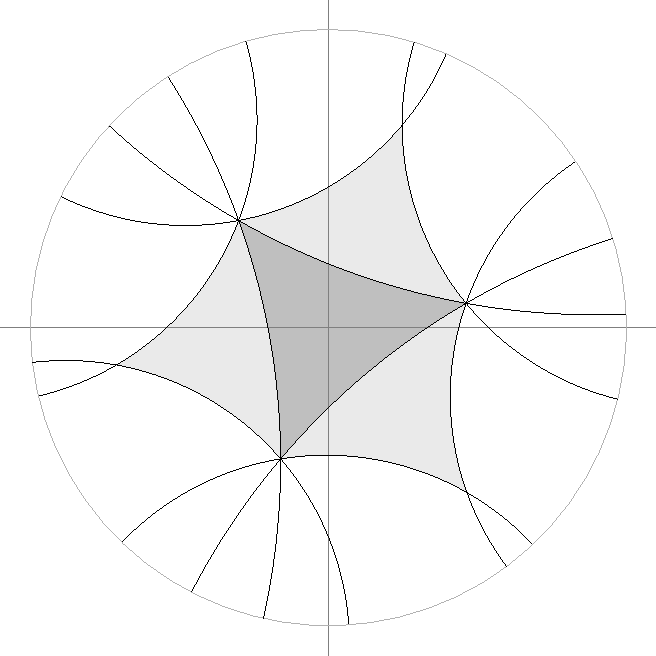
\includegraphics{hyperbolic1}}
\caption{NURBS rendering of $d$-lines in action.}
\label{fig:hyp1}
\end{figure}

\subsection{Rendering `$d$-planes'}


Drawing $d$-lines is interesting in itself but is an already solved 
problem many-times over. What is interesting is the generality the GA
approach provides. Recalling our discussion of the development of
hyperbolic geometry in GA, at no point did we ever assume only 
two-dimensions. We now have the intriguing opportunity to investigate
visualisation algorithms in three-dimensions.

We'll first assume that there is some analogous form to the Poincar\'e
disc representation for three-dimensions. In this case, $d$-lines can
be drawn using a similar method, this time intersecting them with a 
boundary sphere to find the two points of eruption. What would be 
more interesting is attempting to find the form for `$d$-planes'.

The method of defining planes in hyperbolic geometry is identical
to our definition in Euclidean geometry; given four points on the
$d$-plane, $\{ x_1, ..., x_4 \}$, the plane $\Phi$ is defined as
\begin{equation}
\Phi = F_e(x_1) \wedge F_e(x_2) \wedge F_e(x_3) \wedge   F_e(x_4) 
\label{eqn:plane}
\end{equation}
Note we have incorporated the mapping into null-vectors within
the definition. Any point, $p$, which lies on the plane $\Phi$ satisfies
\[
F_e(p) \wedge \Phi = 0
\]

The drawing of $d$-planes is, however, less straight-forward. Firstly we
need to find what shape they are when represented in the Poincar\'e sphere.
Recall that
\[
F_e(x) = \frac{1}{\lambda^2 - x^2} (x^2 + 2\lambda x - \lambda^2\bar{n})
 =  \frac{2\lambda^2}{\lambda^2 - x^2} F(x)
\]
where $F(x)$ is the mapping function for Euclidean geometry. The factor
$(2\lambda^2) / (\lambda^2 - x^2)$ is always scalar for any vector
$x$ and we shall represent it as the function $s(x)$. Hence we can
re-write equation \ref{eqn:plane} as
\begin{eqnarray}
\Phi & = & \bigwedge_{i = 1...4} s(x_i)F(x_i) \\
     & = & \left[\prod_{i = 1...4} s(x_i)\right] \bigwedge_{i = 1...4} F(x_i) \\
     & = & S(x_1, x_2, x_3, x_4) \bigwedge_{i = 1...4} F(x_i) 
%%     & = & \left[\prod_{i = 1...4} s(x_i)\right] \Sigma
\end{eqnarray}

We have expressed $\Phi$ as the product of some scalar function, $S(...)$
of the defining points and the \emph{Euclidean} definition of a sphere. This
allows us to infer that, within the Poincar\'e sphere, a $d$-plane passing
through points $\{x_1, ..., x_4\}$ is represented by a sphere passing
through those same points.

\begin{figure} \centering
\scalebox{0.7}{\includegraphics{dplane}}
\caption{$d$-planes are caps of the corresponding Euclidean sphere.}
\label{fig:dplane}
\end{figure}

It has thus been found, without doing \emph{any} explicit calculations with
the metric, that
$d$-planes are represented in the Poincar\'e sphere by portions of spheres.
This neatly shows the analytical simplicity that this approach provides.
Figure \ref{fig:dplane} shows the
relation between $d$-planes and the corresponding Euclidean sphere.

%This nicely illustrates the analytical power that GA provides us
%with. We have managed to obtain the form of a $d$-plane without
%resorting to complex extreemality calculations and, interestingly,
%without ever explicitly finding the metric. This suggests a powerful
%technique for inverstigating geometries where the geometry is well 
%known but the metric is awkward to deal with. The hyperbolic-tangent
%form for the metric in hyperbolic geometry is tedious to deal with
%analytically but we can infer important properties of the geometry
%intuitively with this approach.

We can find the meet between the associated Euclidean sphere and the
boundary sphere to give the circle of intersection. Inspecting figure
\ref{fig:dplane} we
see that this circle is the edge of the spherical
cap corresponding to the $d$-plane.

The spherical cap forming the $d$-plane can be thought of as the
intersection of the half-space containing the origin and bounded
by the plane of intersection.
The circle of intersection is important since we wish to extract
this \emph{plane} of intersection efficiently. 
If we note that the circle is equivalent to the wedge-product of three
points on the circumference we can form the plane of the circle
by simply wedging the circle with $n$. In summary,
the plane of intersection, $P$ can be found from the $d$-plane $\Phi$ in
the following manner:
\[
P = k (\Phi \vee B) \wedge n
\]
where $B$ is the Euclidean representation of the boundary sphere
and $k$ is some scale factor.

%\begin{figure} \centering
%\scalebox{0.3}{\includegraphics{sphereplane}}
%\caption{$d$-plane spherical cap is intersection of associated sphere and half-space
%to right of plane $P$.}
%\label{fig:sphereplane}
%\end{figure}

Bajaj \emph{et al}\cite{spherecap} provide a method of finding
a suitable set of control points and a NURBS parameter space clipping
curve to draw spherical caps from sphere/half-space intersections.
Their approach gives a set of control points and weights that together
draw a little more than one hemisphere. Circular clipping paths in the 
parameter space are then used to form spherical caps.
This method was used to draw the spherical caps in the implementation.

% \section{Guidelines for Generalising Euclidean Algorithms}
